
\subsection{Pre trained ImageNet CNN}
Here we look to see if we could gain something from CNNs of large networks. The network below is the reference net from Alex Kristevski paper (without the split to be run on two GPUs). The net was trained by [cite] here. 

\begin{figure}[h]
  \centering
  \begin{subfigure}[b]{0.40\textwidth}
   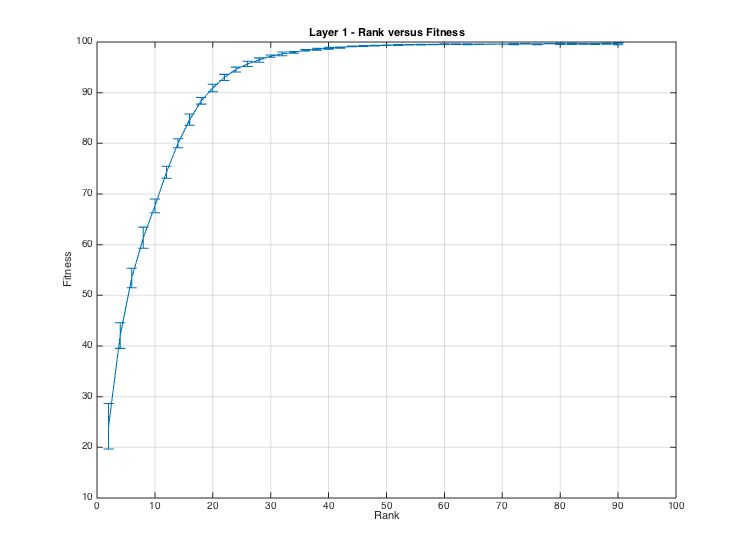
\includegraphics[width=\textwidth]{images/Layer1ImageNet.png}
    \caption{}
  \end{subfigure}
  \begin{subfigure}[b]{0.40\textwidth}
    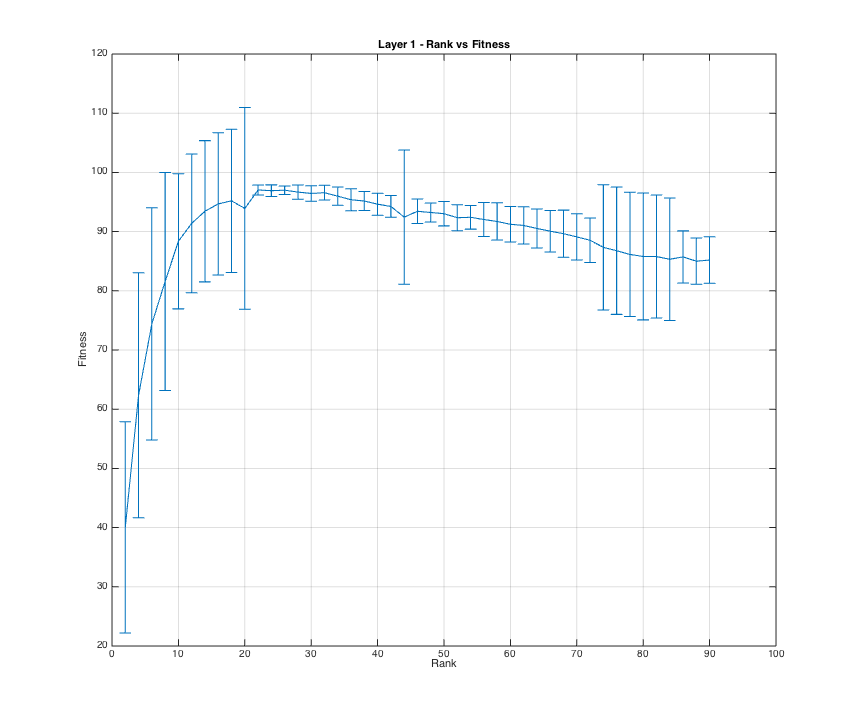
\includegraphics[width=\textwidth]{images/Layer2ImageNet.png}
    \caption{}
  \end{subfigure}
  \caption{ImageNet Layers}
  \label{fig:user_stribution}
\end{figure}

\begin{figure}[h]
  \centering
  \begin{subfigure}[b]{0.40\textwidth}
   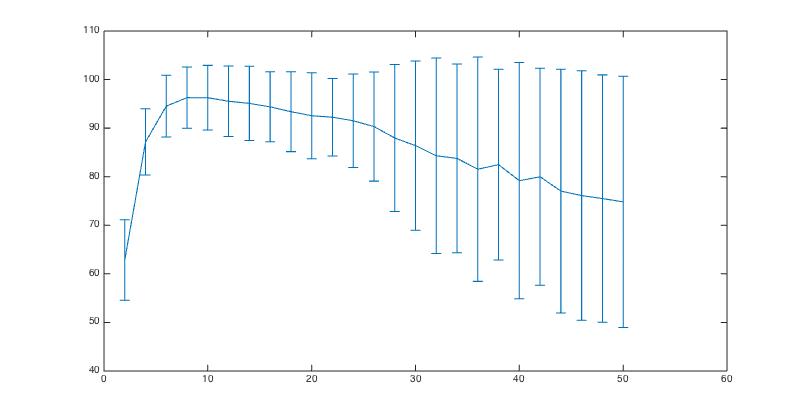
\includegraphics[width=\textwidth]{images/Layer3ImageNet.png}
    \caption{}
  \end{subfigure}
  \begin{subfigure}[b]{0.40\textwidth}
    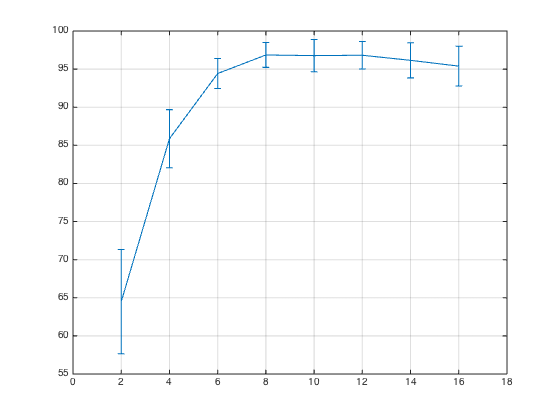
\includegraphics[width=\textwidth]{images/Layer4ImageNet.png}
    \caption{}
  \end{subfigure}
  \caption{ImageNet Layers}
  \label{fig:user_artiststribution}
\end{figure}